%TEMPLATE FOR BEAMER PRESENTATIONS WITH CUSTOM THEME

%TIPS AND TRICKS:
  %If your old presentation based on this library doesn't work, make sure you preamble is up to date

%ASPECT RATIO:
    %4:3  --> 43
    %16:9 --> 169

%HANDOUT MODE
    %1. Add 'handout' to document class options (after aspectratio)
    %2. Put \begin{frame}<handout:0> on a slide you don't want in handout
    %3. For reveals (\only), use '<#|handout:0>', # is the order of the reveal
    %4. For in handout only (e.g. picture in handout, video in presentation),
    %       use: '\only<beamer:0>{command}' (e.g. "dont show up in beamer")

    \documentclass[aspectratio=169, t]{beamer} %frames only
    % \documentclass[aspectratio=169, t, handout]{beamer} %handout version
    % \documentclass[aspectratio=169, t, notes]{beamer}       %frames + notes
    % \documentclass[aspectratio=169, t, notes=only]{beamer}   %only notes

%SOURCE BEAMER THEME LOCALLY OR REMOTELY
    %0 if all .sty and image files located in same directory as .tex
    %1 to use absolute path to reference files in another folder
\newcommand\runlocal{0} %source of beamer theme
\newcommand\usegrid{1} %put 3x3 grid over each slide mimicing matrix display
\newcommand\filledtitle{2} %0: oldschool nasa template with frametitle in line with meatball, 2: sec/subsec above title filled
\newcommand\themecolors{0}    %optional: 1 = ucd colors, other = nasa colors
\newcommand\newfootercenter{0} %center footer text: 0=date, 1=footercenter text
\newcommand\footercenter{new center footer text rather than short title} %use this for SBU message
\newcommand\newfooterleft{0} %left footer text: 0=Author (Institute), 1=leftcenter text
\newcommand\footerleft{new left footer text rather than author/institute}
\newcommand\slidebeforetitle{0} %Title on first slide: 0. (1: have the title on the second slide (e.g. SBU first))
\newcommand\totframesinfoot{0} % 1: total number of frames in footer
\newcommand\titletextwidth{12cm} %width of title text (default 12cm)
\newcommand\titleleftalignfrac{0.24} %left alignment of title textbox as fraction of textwidth (default 0.24)
\newcommand\titleheightfrac{0.775} %fraction hight of title (base?) from top (default 0.775)
\ifnum\runlocal=1%
    %USE BEAMER THEME LOCALLY
    \usetheme{nasa}
\else%
    %USE BEAMER THEME REMOTELY
    %Path to remote beamer template location
    \newcommand\remote{\string~/lib/beamer/nasa}
    \usepackage{\remote/beamerthemenasa}
\fi%

%CUSTOM BEAMER TEMPLATE FORMATTING
\usepackage{caption}  %caption graphics w/o figure environment with '\captionof*{figure}{text}' ('*' omits 'Figure')
% \setbeamertemplate{caption}{\raggedright\insertcaption\par}
\setbeamersize{text margin left=0.25in, text margin right=0.25in} %slide margins

%OTHER PACKAGES
%Graphics
\usepackage{rotate}           %rotate/mirror images
\usepackage[export]{adjustbox} %allow trimming pictures by relative amounts (with 'adjincludegraphics')
%Math
\usepackage{amsmath}          % for formula writing (i.e. 'split', etc)
\usepackage{bbding}           %get \checkmark symbol
\usepackage{cancel}           %"goes to zero" arrow \cancelto{0}{x}
\usepackage{xfrac}            %allows slated and side fractions
% %Movies
% \usepackage{media9}         %embed flash multimedia, won't work after 2020
% % \usepackage{multimedia}       %allows embedded movies REMOVED TO AVOID CONFLICT WITH MEDIA9
% % \usepackage{movie15}          %play un-embedded movies with external player
% \usepackage{animate}          %animate series of stills like a gif
% \usepackage{graphicx}         %allows saving movies (???)
% %Formatting
% \usepackage{framed}           %allows shaded text
% \usepackage{soul}             %text highlighting
% \usepackage{markdown} %use markdown syntax with \begin{markdown}
% \markdownSetup{
%   renderers = {
%     link     = {#1},        % Render a link as the link label.
%     emphasis = {\emph{#1}}, % Render emphasis using `\emph`.
%   }
% }

% %TIKZ
% \usepackage{tikz}             %for creating vector graphics diagrams
% \usetikzlibrary{backgrounds}  %put backgrounds behind tikz figures
% \usetikzlibrary{calc}         %perform calculations within $$
% \usetikzlibrary{positioning}  %position tikz elements
% \usetikzlibrary{angles}       %label angles between lines with arcs
% \usetikzlibrary{quotes}       %Put angle label in quotes
% \usetikzlibrary{shapes}       %all of the shapes
% \usetikzlibrary{arrows}       %arrow styles
% \usetikzlibrary{fit}          %fit nodes in boxes
% \usetikzlibrary{patterns}     %allow cross hatching

% \usepackage[beamer, customcolors]{hf-tikz}%for boxed equations
% \usepackage[mode=buildnew]{standalone}% requires -shell-escape
%   % compile with `pdflatex -shell-escape main` or `xelatex  -shell-escape main`


% %CODE LISTING SYNTAX COLORING
% \newcommand\whiteback{0} %code listing background color (0: black, 1: white)
% %%%%%%%%%%%%%%%%%%%%%%%%%%%%%%%%%%%%%%%%%%%%%%%
%CODE LISTING SYNTAX COLORING
%Source code listings from files and present them using Sublime Text
%syntax coloring.

%CALL LISTING PACKAGE IN SEPARATE BEAMER.TEX WITH:
%\newcommand\whiteback{0} %code listing background color (0: black, 1: white)
%%%%%%%%%%%%%%%%%%%%%%%%%%%%%%%%%%%%%%%%%%%%%%%%
%CODE LISTING SYNTAX COLORING
%Source code listings from files and present them using Sublime Text
%syntax coloring.

%CALL LISTING PACKAGE IN SEPARATE BEAMER.TEX WITH:
%\newcommand\whiteback{0} %code listing background color (0: black, 1: white)
%%%%%%%%%%%%%%%%%%%%%%%%%%%%%%%%%%%%%%%%%%%%%%%%
%CODE LISTING SYNTAX COLORING
%Source code listings from files and present them using Sublime Text
%syntax coloring.

%CALL LISTING PACKAGE IN SEPARATE BEAMER.TEX WITH:
%\newcommand\whiteback{0} %code listing background color (0: black, 1: white)
%\input{\string~/lib/beamer/codelisting}


\usepackage{color}     %make custom colors for syntax coloring
\usepackage{listings}  %allows code listings
\usepackage{textcomp}  %allows apostrophes to be straight (unidirectional)
% \usepackage{framed}
% \usepackage{caption}
\usepackage{bm}
\usepackage{tcolorbox}        %use for code listing color definitions
\tcbuselibrary{listings}      %allow color defenitions in code listings

\captionsetup[lstlisting]{font={small,tt}}

%Custom Colors
\definecolor{mygreen}{rgb}{0,0.6,0}
\definecolor{mygray}{rgb}{0.5,0.5,0.5}
\definecolor{mymauve}{rgb}{0.58,0,0.82}

\definecolor{sublimeblack}{HTML}{272822}
\definecolor{sublimered}{HTML}{F92672}
\definecolor{sublimeblue}{HTML}{66D9EF}
\definecolor{sublimeyellow}{HTML}{E6DB74}
\definecolor{sublimegrey}{HTML}{75715E}
\definecolor{sublimegreen}{HTML}{66CC33}
\definecolor{sublimeorange}{HTML}{FD971F}
\definecolor{sublimepurple}{HTML}{AE81FF}


%White or Black background toggle
% \newcommand\whiteback{0}
\ifnum\whiteback=1%
  %White Background
  \newcommand\backclr{white}
  \newcommand\txtclr{\color{black}}
  \newcommand\comclr{\color{mygreen}}
  \newcommand\keyclr{\color{blue}}
  \newcommand\ndkeyclr{\color{sublimered}}
  \newcommand\strclr{\color{mymauve}}
  \newcommand\frameon{single} %single-frame box around code
\else
  %Black Background (like SublimeText)
  \newcommand\backclr{sublimeblack}
  \newcommand\txtclr{\color{white}}
  \newcommand\comclr{\color{sublimegrey}}
  \newcommand\keyclr{\color{sublimeblue}}
  \newcommand\ndkeyclr{\color{sublimered}}
  \newcommand\strclr{\color{sublimeyellow}}
  \newcommand\frameon{false} %no frame for black background
\fi


%Listing Style
\lstdefinestyle{mystyle}{%
  % backgroundcolor=\backclr,   % choose the background color; you must add \usepackage{color} or \usepackage{xcolor}
  basicstyle=\ttfamily\txtclr\scriptsize, % the SIZE OF THE FONTS that are used for the code
  breakatwhitespace=false,         % sets if automatic breaks should only happen at whitespace
  % breaklines=true,                 % sets automatic line breaking
  captionpos=b,                    % sets the caption-position to bottom
  commentstyle=\comclr,            % comment color
  deletekeywords={...},            % if you want to delete keywords from the given language
  escapeinside={\%*}{*)},          % if you want to add LaTeX within your code
  extendedchars=true,              % lets you use non-ASCII characters; for 8-bits encodings only, does not work with UTF-8
  frame=\frameon,                  % adds a frame around the code
  keepspaces=true,                 % keeps spaces in text, useful for keeping indentation of code (possibly needs columns=flexible)
  columns=flexible,
  otherkeywords={zip,enumerate,True,False,None,...},  %add words to be highlighted
  keywordstyle=\keyclr,            % keyword (e.g. 'print') color
  language=Python,                 % the language of the code
  upquote=true,                    % make apostrophes straight (unidirectional)
  alsoletter={<>=-+*/!},            % to avoid coloring operators when they're not
  ndkeywords={=,+,-,*,**,/,+=,*=,-=,/=,<=,>=,==,!=,<,>,... },  % operator keywords
  ndkeywordstyle=\ndkeyclr,         % style of operator keywords
  numbers=left,                    % where to put the line-numbers; possible values are (none, left, right)
  numbersep=5pt,                   % how far the line-numbers are from the code
  numberstyle=\tiny\color{mygray}, % line-number style: size, color
  rulecolor=\color{black},         % if not set, the frame-color may be changed on line-breaks within not-black text (e.g. comments (green here))
  showspaces=false,                % show spaces everywhere adding particular underscores; it overrides 'showstringspaces'
  showstringspaces=false,          % underline spaces within strings only
  showtabs=false,                  % show tabs within strings adding particular underscores
  stepnumber=1,                    % the step between two line-numbers. If it's 1, each line will be numbered
  stringstyle=\strclr,             % string color
  tabsize=4,                       % sets default tabsize
}


%Function that calls listing of specific file with custom coloring
  %first input is filename to list
  %next two inputs are start and end line numbers
    %(use 0 and large number for all lines)
\newcommand\mylisting[3]{
  \tcbinputlisting{
        listing file=#1,
        arc=0pt,
        top=0mm,
        bottom=0mm,
        left=0mm,
        right=0mm,
        boxrule=0pt,
        colback=\backclr,
        listing only,
        listing options={
                            style=mystyle,            %use custom style
                            firstline=#2,lastline=#3, %lines of code to use
                            firstnumber=#2,           %same numbering as script
                        },
        hbox
      }
      }



\usepackage{color}     %make custom colors for syntax coloring
\usepackage{listings}  %allows code listings
\usepackage{textcomp}  %allows apostrophes to be straight (unidirectional)
% \usepackage{framed}
% \usepackage{caption}
\usepackage{bm}
\usepackage{tcolorbox}        %use for code listing color definitions
\tcbuselibrary{listings}      %allow color defenitions in code listings

\captionsetup[lstlisting]{font={small,tt}}

%Custom Colors
\definecolor{mygreen}{rgb}{0,0.6,0}
\definecolor{mygray}{rgb}{0.5,0.5,0.5}
\definecolor{mymauve}{rgb}{0.58,0,0.82}

\definecolor{sublimeblack}{HTML}{272822}
\definecolor{sublimered}{HTML}{F92672}
\definecolor{sublimeblue}{HTML}{66D9EF}
\definecolor{sublimeyellow}{HTML}{E6DB74}
\definecolor{sublimegrey}{HTML}{75715E}
\definecolor{sublimegreen}{HTML}{66CC33}
\definecolor{sublimeorange}{HTML}{FD971F}
\definecolor{sublimepurple}{HTML}{AE81FF}


%White or Black background toggle
% \newcommand\whiteback{0}
\ifnum\whiteback=1%
  %White Background
  \newcommand\backclr{white}
  \newcommand\txtclr{\color{black}}
  \newcommand\comclr{\color{mygreen}}
  \newcommand\keyclr{\color{blue}}
  \newcommand\ndkeyclr{\color{sublimered}}
  \newcommand\strclr{\color{mymauve}}
  \newcommand\frameon{single} %single-frame box around code
\else
  %Black Background (like SublimeText)
  \newcommand\backclr{sublimeblack}
  \newcommand\txtclr{\color{white}}
  \newcommand\comclr{\color{sublimegrey}}
  \newcommand\keyclr{\color{sublimeblue}}
  \newcommand\ndkeyclr{\color{sublimered}}
  \newcommand\strclr{\color{sublimeyellow}}
  \newcommand\frameon{false} %no frame for black background
\fi


%Listing Style
\lstdefinestyle{mystyle}{%
  % backgroundcolor=\backclr,   % choose the background color; you must add \usepackage{color} or \usepackage{xcolor}
  basicstyle=\ttfamily\txtclr\scriptsize, % the SIZE OF THE FONTS that are used for the code
  breakatwhitespace=false,         % sets if automatic breaks should only happen at whitespace
  % breaklines=true,                 % sets automatic line breaking
  captionpos=b,                    % sets the caption-position to bottom
  commentstyle=\comclr,            % comment color
  deletekeywords={...},            % if you want to delete keywords from the given language
  escapeinside={\%*}{*)},          % if you want to add LaTeX within your code
  extendedchars=true,              % lets you use non-ASCII characters; for 8-bits encodings only, does not work with UTF-8
  frame=\frameon,                  % adds a frame around the code
  keepspaces=true,                 % keeps spaces in text, useful for keeping indentation of code (possibly needs columns=flexible)
  columns=flexible,
  otherkeywords={zip,enumerate,True,False,None,...},  %add words to be highlighted
  keywordstyle=\keyclr,            % keyword (e.g. 'print') color
  language=Python,                 % the language of the code
  upquote=true,                    % make apostrophes straight (unidirectional)
  alsoletter={<>=-+*/!},            % to avoid coloring operators when they're not
  ndkeywords={=,+,-,*,**,/,+=,*=,-=,/=,<=,>=,==,!=,<,>,... },  % operator keywords
  ndkeywordstyle=\ndkeyclr,         % style of operator keywords
  numbers=left,                    % where to put the line-numbers; possible values are (none, left, right)
  numbersep=5pt,                   % how far the line-numbers are from the code
  numberstyle=\tiny\color{mygray}, % line-number style: size, color
  rulecolor=\color{black},         % if not set, the frame-color may be changed on line-breaks within not-black text (e.g. comments (green here))
  showspaces=false,                % show spaces everywhere adding particular underscores; it overrides 'showstringspaces'
  showstringspaces=false,          % underline spaces within strings only
  showtabs=false,                  % show tabs within strings adding particular underscores
  stepnumber=1,                    % the step between two line-numbers. If it's 1, each line will be numbered
  stringstyle=\strclr,             % string color
  tabsize=4,                       % sets default tabsize
}


%Function that calls listing of specific file with custom coloring
  %first input is filename to list
  %next two inputs are start and end line numbers
    %(use 0 and large number for all lines)
\newcommand\mylisting[3]{
  \tcbinputlisting{
        listing file=#1,
        arc=0pt,
        top=0mm,
        bottom=0mm,
        left=0mm,
        right=0mm,
        boxrule=0pt,
        colback=\backclr,
        listing only,
        listing options={
                            style=mystyle,            %use custom style
                            firstline=#2,lastline=#3, %lines of code to use
                            firstnumber=#2,           %same numbering as script
                        },
        hbox
      }
      }



\usepackage{color}     %make custom colors for syntax coloring
\usepackage{listings}  %allows code listings
\usepackage{textcomp}  %allows apostrophes to be straight (unidirectional)
% \usepackage{framed}
% \usepackage{caption}
\usepackage{bm}
\usepackage{tcolorbox}        %use for code listing color definitions
\tcbuselibrary{listings}      %allow color defenitions in code listings

\captionsetup[lstlisting]{font={small,tt}}

%Custom Colors
\definecolor{mygreen}{rgb}{0,0.6,0}
\definecolor{mygray}{rgb}{0.5,0.5,0.5}
\definecolor{mymauve}{rgb}{0.58,0,0.82}

\definecolor{sublimeblack}{HTML}{272822}
\definecolor{sublimered}{HTML}{F92672}
\definecolor{sublimeblue}{HTML}{66D9EF}
\definecolor{sublimeyellow}{HTML}{E6DB74}
\definecolor{sublimegrey}{HTML}{75715E}
\definecolor{sublimegreen}{HTML}{66CC33}
\definecolor{sublimeorange}{HTML}{FD971F}
\definecolor{sublimepurple}{HTML}{AE81FF}


%White or Black background toggle
% \newcommand\whiteback{0}
\ifnum\whiteback=1%
  %White Background
  \newcommand\backclr{white}
  \newcommand\txtclr{\color{black}}
  \newcommand\comclr{\color{mygreen}}
  \newcommand\keyclr{\color{blue}}
  \newcommand\ndkeyclr{\color{sublimered}}
  \newcommand\strclr{\color{mymauve}}
  \newcommand\frameon{single} %single-frame box around code
\else
  %Black Background (like SublimeText)
  \newcommand\backclr{sublimeblack}
  \newcommand\txtclr{\color{white}}
  \newcommand\comclr{\color{sublimegrey}}
  \newcommand\keyclr{\color{sublimeblue}}
  \newcommand\ndkeyclr{\color{sublimered}}
  \newcommand\strclr{\color{sublimeyellow}}
  \newcommand\frameon{false} %no frame for black background
\fi


%Listing Style
\lstdefinestyle{mystyle}{%
  % backgroundcolor=\backclr,   % choose the background color; you must add \usepackage{color} or \usepackage{xcolor}
  basicstyle=\ttfamily\txtclr\scriptsize, % the SIZE OF THE FONTS that are used for the code
  breakatwhitespace=false,         % sets if automatic breaks should only happen at whitespace
  % breaklines=true,                 % sets automatic line breaking
  captionpos=b,                    % sets the caption-position to bottom
  commentstyle=\comclr,            % comment color
  deletekeywords={...},            % if you want to delete keywords from the given language
  escapeinside={\%*}{*)},          % if you want to add LaTeX within your code
  extendedchars=true,              % lets you use non-ASCII characters; for 8-bits encodings only, does not work with UTF-8
  frame=\frameon,                  % adds a frame around the code
  keepspaces=true,                 % keeps spaces in text, useful for keeping indentation of code (possibly needs columns=flexible)
  columns=flexible,
  otherkeywords={zip,enumerate,True,False,None,...},  %add words to be highlighted
  keywordstyle=\keyclr,            % keyword (e.g. 'print') color
  language=Python,                 % the language of the code
  upquote=true,                    % make apostrophes straight (unidirectional)
  alsoletter={<>=-+*/!},            % to avoid coloring operators when they're not
  ndkeywords={=,+,-,*,**,/,+=,*=,-=,/=,<=,>=,==,!=,<,>,... },  % operator keywords
  ndkeywordstyle=\ndkeyclr,         % style of operator keywords
  numbers=left,                    % where to put the line-numbers; possible values are (none, left, right)
  numbersep=5pt,                   % how far the line-numbers are from the code
  numberstyle=\tiny\color{mygray}, % line-number style: size, color
  rulecolor=\color{black},         % if not set, the frame-color may be changed on line-breaks within not-black text (e.g. comments (green here))
  showspaces=false,                % show spaces everywhere adding particular underscores; it overrides 'showstringspaces'
  showstringspaces=false,          % underline spaces within strings only
  showtabs=false,                  % show tabs within strings adding particular underscores
  stepnumber=1,                    % the step between two line-numbers. If it's 1, each line will be numbered
  stringstyle=\strclr,             % string color
  tabsize=4,                       % sets default tabsize
}


%Function that calls listing of specific file with custom coloring
  %first input is filename to list
  %next two inputs are start and end line numbers
    %(use 0 and large number for all lines)
\newcommand\mylisting[3]{
  \tcbinputlisting{
        listing file=#1,
        arc=0pt,
        top=0mm,
        bottom=0mm,
        left=0mm,
        right=0mm,
        boxrule=0pt,
        colback=\backclr,
        listing only,
        listing options={
                            style=mystyle,            %use custom style
                            firstline=#2,lastline=#3, %lines of code to use
                            firstnumber=#2,           %same numbering as script
                        },
        hbox
      }
      }








%%%%%%%%%%%%%%%%%%%%%%%%%%%%%%%%%%%%%%%%%%%%%%%%%%%%%%%%%%%%%%%%%%%%%%%%
%%% TITLE PAGE INFO %%%%%%%%%%%%%%%%%%%%%%%%%%%%%%%%%%%%%%%%%%%%%%%%%%%%
%%%%%%%%%%%%%%%%%%%%%%%%%%%%%%%%%%%%%%%%%%%%%%%%%%%%%%%%%%%%%%%%%%%%%%%%

%title, author, institute have the option for an additional [short title] that will be displayed in the footer
  %default short title is title
\title[Short Title]{Presentation Title Here}
\subtitle{With A Subtitle Here}
\author{Logan Halstrom}
\institute{NASA}
\date{\today}

%LOAD IMAGES FOR TITLE SLIDE
%Paths to images:
\ifnum\runlocal=1%
    \newcommand\EGlogo{Images/EG_Logo.png}
    \newcommand\SLSpic{Images/Orion_SLS_trim.png}
\else%
    \newcommand\EGlogo{\remote/Images/EG_Logo.png}
    % \newcommand\SLSpic{\remote/Images/Orion_SLS_trim.png}
    \newcommand\SLSpic{\remote/Images/SLS_Orange.png}
\fi%
%ADD IMAGES TO TITTLE SLIDE
\addtobeamertemplate{title page}
{
%Not sure how positioning works, (-1cm,0cm for upper left corner apparently)
\begin{textblock*}{0cm}(-0.5cm,0.5cm) %Textbox witdh, then coords of center
\includegraphics[scale=0.5]{\EGlogo}
\end{textblock*}

% \begin{textblock*}{0cm}(0.84\textwidth,0.25cm)
% \includegraphics[height=\textheight]{\SLSpic}
% \end{textblock*}
\begin{textblock*}{0cm}(0.7\textwidth,0.25cm)
\includegraphics[height=\textheight]{\SLSpic}
\end{textblock*}
}

%%%%%%%%%%%%%%%%%%%%%%%%%%%%%%%%%%%%%%%%%%%%%%%%%%%%%%%%%%%%%%%%%%%%%%%%
%%% START DOCUMENT %%%%%%%%%%%%%%%%%%%%%%%%%%%%%%%%%%%%%%%%%%%%%%%%%%%%%
%%%%%%%%%%%%%%%%%%%%%%%%%%%%%%%%%%%%%%%%%%%%%%%%%%%%%%%%%%%%%%%%%%%%%%%%

\begin{document}

%%%%%%%%%%%%%%%%%%%%%%%%%%%%%%%%%%%%%%%%%%%%%%%%%%%%%%%%%%%%%%%%%%%%%%%%
%%% MAKE TITLE PAGE %%%%%%%%%%%%%%%%%%%%%%%%%%%%%%%%%%%%%%%%%%%%%%%%%%%%
%%%%%%%%%%%%%%%%%%%%%%%%%%%%%%%%%%%%%%%%%%%%%%%%%%%%%%%%%%%%%%%%%%%%%%%%

%%% OPTION FOR PAGE BEFORE TITLE (E.G. SBU NOTICE, ETC)
\ifnum\slidebeforetitle=1
  \vspace{-0.1in}
  \begin{frame}
  \begin{columns}
  \column{1.15\textwidth}
  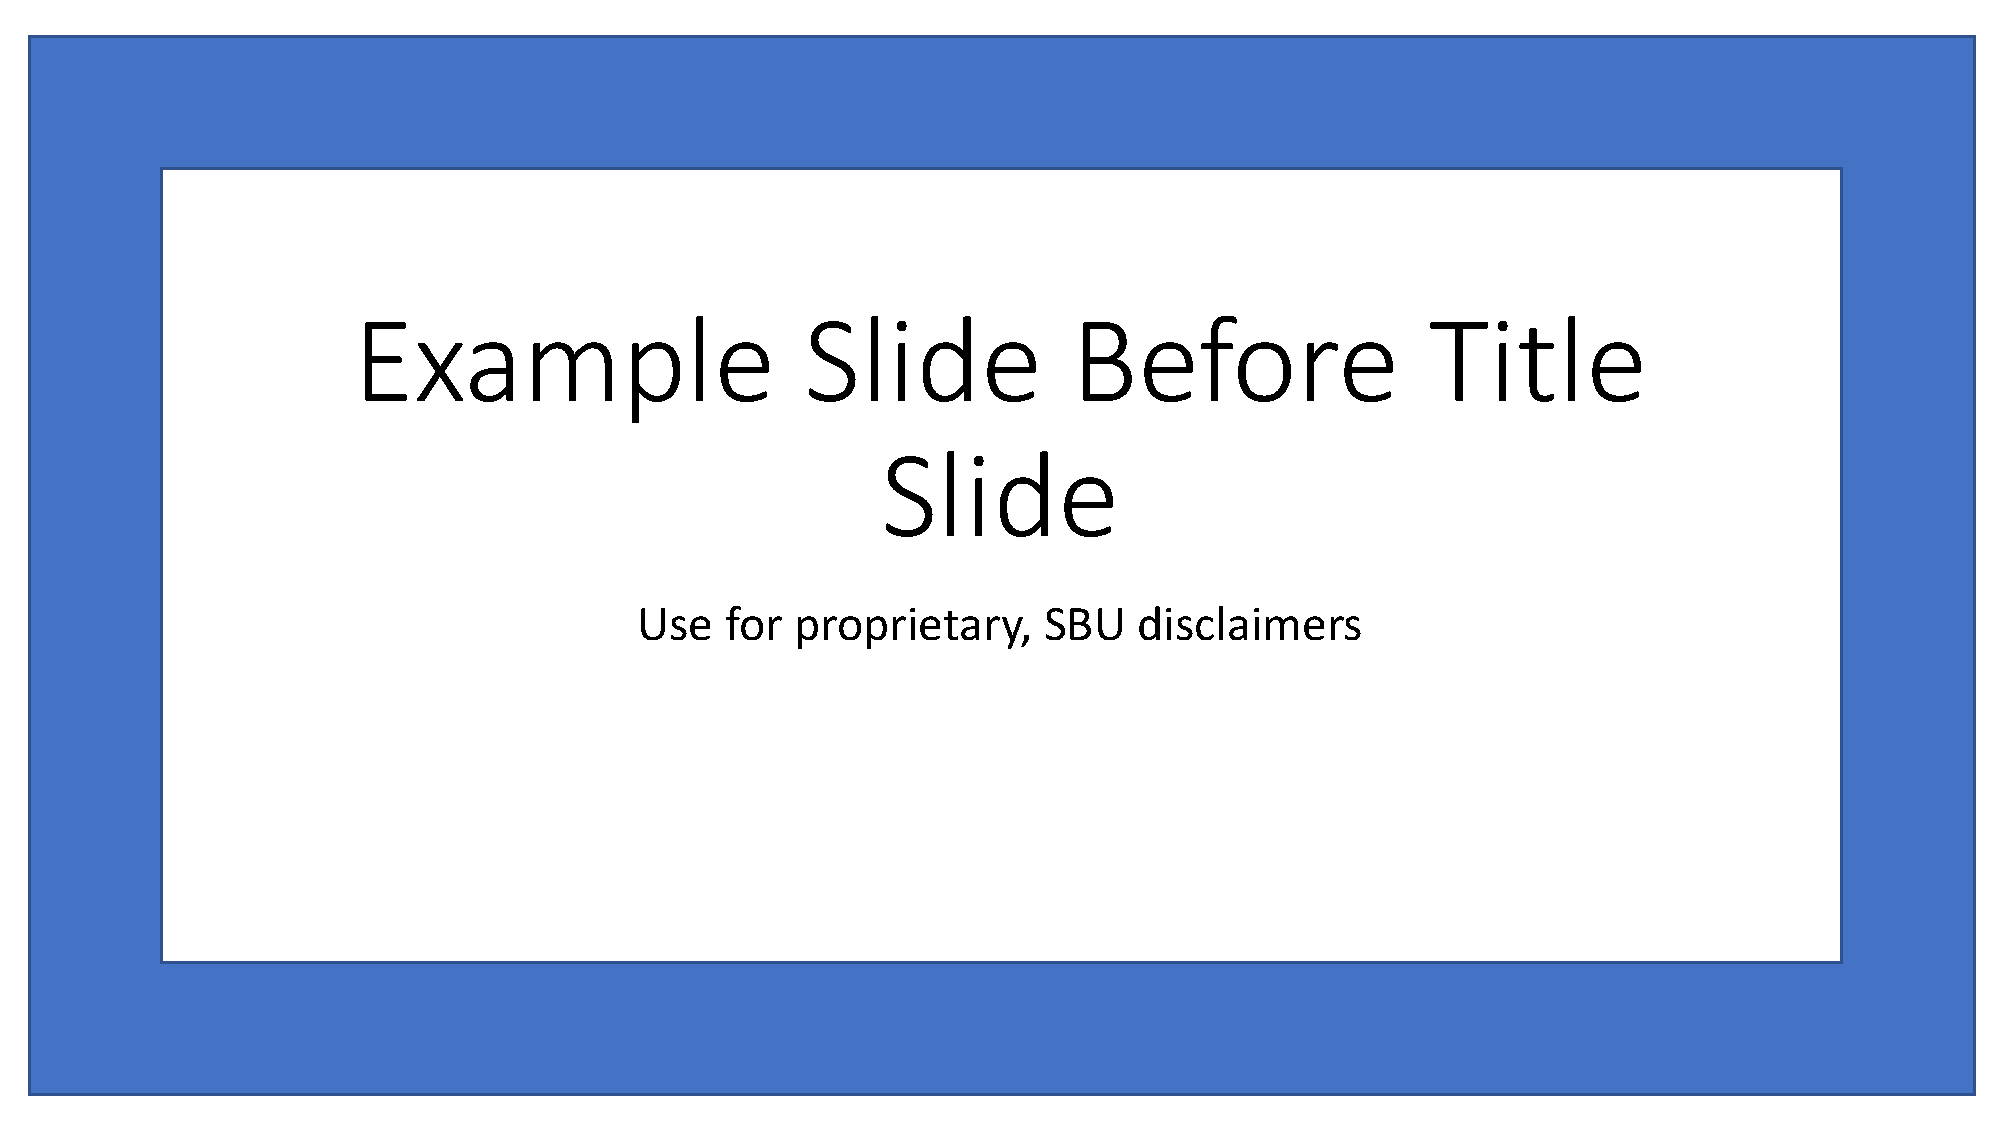
\includegraphics[width=1.0\textwidth,page=1]{Images/pre-titleslide.pdf}
  \end{columns}
  \end{frame}
\fi

%STANDARD TITLE PAGE
\begin{frame}
\titlepage
\end{frame}

%%%%%%%%%%%%%%%%%%%%%%%%%%%%%%%%%%%%%%%%%%%%%%%%%%%%%%%%%%%%%%%%%%%%%%%%
%%% PRESENTATION OUTLINE %%%%%%%%%%%%%%%%%%%%%%%%%%%%%%%%%%%%%%%%%%%%%%%
%%%%%%%%%%%%%%%%%%%%%%%%%%%%%%%%%%%%%%%%%%%%%%%%%%%%%%%%%%%%%%%%%%%%%%%%

%SHOW OVERALL OUTLINE AT BEGINNING
%Use * to leave sections out of overview (e.g. \section*{Backup})
\begin{frame}\frametitle{Outline}
\tableofcontents
\end{frame}

%SHOW OUTLINE OF EACH SECTION AS EACH SECTION IS REACHED
\AtBeginSection[]
{
  \ifnum \thesection>1 %don't have outine before first sect (redundant)
  \begin{frame}
  \frametitle{Outline for Section \thesection}
  \tableofcontents[currentsection] %show sections and subsections
  % \tableofcontents[currentsection, hideallsubsections] %only show sections
  \end{frame}
\else
\fi
}

% %SHOW OUTLINE OF EACH SUBSECTION AS EACH SUBSECTION IS REACHED
% \AtBeginSubsection[]
% {
% \ifnum \thesubsection>1 %don't have outine before first sect (redundant)
%   \begin{frame}
%   \frametitle{Outline for Section \thesection.\thesubsection}
%   \tableofcontents[currentsubsection]
%   \end{frame}
% \else
% \fi
% }
%%%%%%%%%%%%%%%%%%%%%%%%%%%%%%%%%%%%%%%%%%%%%%%%%%%%%%%%%%%%%%%%%%%%%%%%
%%% GENERAL SLIDES %%%%%%%%%%%%%%%%%%%%%%%%%%%%%%%%%%%%%%%%%%%%%%%%%%%%%
%%%%%%%%%%%%%%%%%%%%%%%%%%%%%%%%%%%%%%%%%%%%%%%%%%%%%%%%%%%%%%%%%%%%%%%%




%===============================================================================
\section{Section 1}\label{Sec1}
%===============================================================================





%===============================================================================
\subsection{Subsection 1a}\label{Sub1a}



%%%%%%%%%%%%%%%%%%%%%%%%%%%
\begin{frame}\frametitle{Title: Section \thesection Subsection \thesubsection}
% \framesubtitle{Subtitle}
Demonstrates sections and subsections
\end{frame}

%===============================================================================
\subsection{Subsection 1b}

%%%%%%%%%%%%%%%%%%%%%%%%%%%
\begin{frame}\frametitle{Title: Section \thesection Subsection \thesubsection}
  Demonstrates sections and subsections again
\end{frame}

%===============================================================================
\section{Example Slides}
%===============================================================================



%===============================================================================
\subsection{Lists}


%%%%%%%%%%%%%%%%%%%%%%%%%%%%%%%%%%%%
\begin{frame}\frametitle{Itemized Lists}
%ITEMIZED LIST DEMO

List Title
\begin{itemize}
    \item First bullet
    \item Second bullet
    \begin{itemize}
        \item First subbullet
        \begin{itemize}
            \item First subsubbullet
            \item Second subsubbullet
        \end{itemize}
        \item Second subbullet
    \end{itemize}
    \item Third bullet
\end{itemize}
\end{frame}



%%%%%%%%%%%%%%%%%%%%%%%%%%%
\begin{frame} \frametitle{Enumerated Lists}
  %ENUMERATED LIST DEMO

  Enumerated (Numbered) List Test
  \begin{enumerate}
      \item Item 1
      \item Item 2
      \begin{enumerate}[i)] %label with lowercase roman numeral with right parenthesis
          \item Subitem 1
          \item Subitem 2
      \end{enumerate}
      \item Item 3
  \end{enumerate}
  \end{frame}


%===============================================================================
\subsection{Block Text}


%%%%%%%%%%%%%%%%%%%%%%%%%%%%%%%%%%%%
\begin{frame}\frametitle{Block Demo}
  %TEXT BLOCK DEMO
  %-------------------------------------
  %   title                             |
  %                                     |
  %      ________________________       |
  %     | text block             |      |
  %     |________________________|      |
  %                                     |
  %      ________________________       |
  %     | text block             |      |
  %     |________________________|      |
  %-------------------------------------

  \begin{block}{Block Demonstration}
You can have a main idea as a title of the block, then discuss it as a paragraph below, with nice colors.
\end{block}


\begin{block}{Block List}
    \begin{itemize}
      \item You can also have a list in the block
        \begin{itemize}
          \item Overall idea with multiple options
          \item Some other reason
          \item Even more reasons
        \end{itemize}
      \item That way you can keep your list concept separate from the previous sentence concept
      \item Hopefully, this looks more organized
    \end{itemize}
\end{block}
\end{frame}



%===============================================================================
\subsection{Pictures}


%%%%%%%%%%%%%%%%%%%%%%%%%%%
\begin{frame}\frametitle{Pictures In Columns}

\begin{columns}[b]
\column{0.5\textwidth}
  \begin{center}
    Title text for Pic 1
    
\includegraphics[width=\textwidth]{Images/Orion_logo.png}
  \end{center}

\column{0.5\textwidth}
  \begin{center}
    Title text for Pic 2
    
\includegraphics[width=\textwidth]{Images/EG_Logo.png}
  \end{center}
\end{columns}
\end{frame}



  %%%%%%%%%%%%%%%%%%%%%%%%%%%%%%%%%%%%
  \begin{frame}\frametitle{Pictures Above Text Block}
    % \vspace{-0.475in}

    %-------------------------------------
    %   title                             |
    %       ______         ______         |
    %      |      |       |      |        |
    %      |  pic |       |  pic |        |
    %      |______|       |______|        |
    %      ________________________       |
    %     | text block             |      |
    %     |________________________|      |
    %-------------------------------------

    \begin{columns}[t]


    \column{0.5\textwidth}

    % \vspace{-0.25in}
    \begin{center}
      %[trim=left bottom right top, clip]
      
\includegraphics[trim=0 0 0 0, clip, width=1.0\textwidth]{Images/Orion_logo.png}
      \captionof*{figure}{ Caption for Figure 1 }
      \end{center}


    \column{0.5\textwidth}

    % \vspace{-0.25in}


    \begin{center}
      
\includegraphics[trim=0 0 0 0, clip, width=1.0\textwidth]{Images/NASA_Meatball.png}
      \vspace{-1.2cm}
      \captionof{figure}{ Caption for Figure 2 }

    \end{center}


    \end{columns}


  % \vspace{-0.1in}



    \begin{block}{}
      \begin{itemize}
        \item Descriptive text about pictures
      \end{itemize}
    \end{block}

    \end{frame}



%%%%%%%%%%%%%%%%%%%%%%%%%%%%%%%%%%%%
\begin{frame}\frametitle{2 Column: Left Picture, Right Text Blocks}
  % \vspace{-0.475in}

  %-------------------------------------
  %   title                             |
  %                    ________         |
  %                   | text   |        |
  %       ______      |  block |        |
  %      |      |     |________|        |
  %      |  pic |      ________         |
  %      |______|     | text   |        |
  %                   |  block |        |
  %                   |________|        |
  %-------------------------------------



  \begin{columns}[t]


  \column{0.5\textwidth}

  % \vspace{-0.25in}
  \begin{center}
    %[trim=left bottom right top, clip]
    
\includegraphics[trim=0 0 0 0, clip, width=1.0\textwidth]{Images/Orion_logo.png}
    \vspace{-0.5cm}
    \captionof*{figure}{ Caption for Figure 2 }
    \end{center}


  \column{0.5\textwidth}

  \begin{block}{Text Block 1}
    \begin{itemize}
      \item Text 1
    \end{itemize}
  \end{block}

  \vspace{-0.1in}

  \begin{block}{Text Block 2}
    \begin{itemize}
      \item Text 2
    \end{itemize}
  \end{block}


  \end{columns}




  \end{frame}














%CALL THIS AT BEGINNING OF BACKUP SLIDES TO EXCLUDE FROM TOTAL COUNT
\backupbegin

%===============================================================================
\section*{Backup}
%===============================================================================
%* makes backup not appear in table of contents

%%%%%%%%%%%%%%%%%%%%%%%%%%%
\begin{frame}\frametitle{Backup}
\end{frame}

%===============================================================================
\subsection*{Backup Section Name}




%===============================================================================
\subsection*{References}

%%%%%%%%%%%%%%%%%%%%%%%%%%%
\begin{frame}\frametitle{Example Citations}
\cite{knacke1968apollo}
\cite{mckinney2013boeing}
\cite{adams2009mars}
\cite{ray2015pendulum}
\cite{ali2017orion}
\cite{anderson2017subscale}

\end{frame}

%%%%%%%%%%%%%%%%%%%%%%%%%%%
\begin{frame}[allowframebreaks]\frametitle{References}
%list all references cited with "\cite"
%'allowframebreaks' splits content over multiple slides
        \bibliographystyle{ieeetr} %style of references
        \bibliography{nasa}        %source .bib file
\end{frame}


%CALL THIS AT END OF BACKUP TO COUNT SLIDES AGAIN
\backupend


\end{document}
